\section{The Large Hadron Collider}
The CERN Large Hadron Collider (LHC) is a two-ring superconducting
accelerator and collider with 27 km of circumference, which is located
in the tunnel constructed for the CERN Large Electron-Positron
Collider (LEP). The tunnel lies between 45 m and 170 m below the
surface on an incliend plane (1.41\% slope) towards Lake L\`eman and
spans between the French and Swiss border close to Geneva. The layout
of the tunnel is such that contains 8 arc sections that spans most of
the circumference and 8 straight sections where the experimental halls
are located. 

The LHC is a particle-particle collider -- in its most common
configuration it collides protons -- with a designed center-of-mass
energy of 14\TeV. In order to achieve such high energies, the LHC uses
the existing CERN facilities to gradually increase the energy of the
protons. Everything starts with a bottle of compressed hydrogen gas,
then, hydrogen atoms are fed into the source chamber of the linear
accelerator, where an electric field strips off their
electrons. The resulting protons are then injected into the linear
accelaretor, Linac 2, which is the first step in the
accelerator chain and boosts the
protons energy up to 50\MeV. The accelated proton beam is then divided
into 4 (to increase its intensity) and enters the second stage of
acceleration, this occurs in the Proton Synchroton Booster (PSB),
where protons are now accelerated to 1.4\GeV. Subsequently, the proton beam is
recombined and sent to the Proton Synchrotron (PS), which increases
the energy to 25\GeV, followed by the Super Proton Synchrotron (SPS),
which brings the beam energy to 450\GeV.

Finally, the proton beam is transfered to the two beam pipes of the
LHC. The beams circulate in opposite directions. The LHC filling time
is 4 minutes and 20 seconds, but it takes around 20 minutes for the
protons to reach their maximum energy. Figure~\ref{fig:cernAcc} shows
the CERN accelerator complex just described.
\begin{figure}
 \centering
 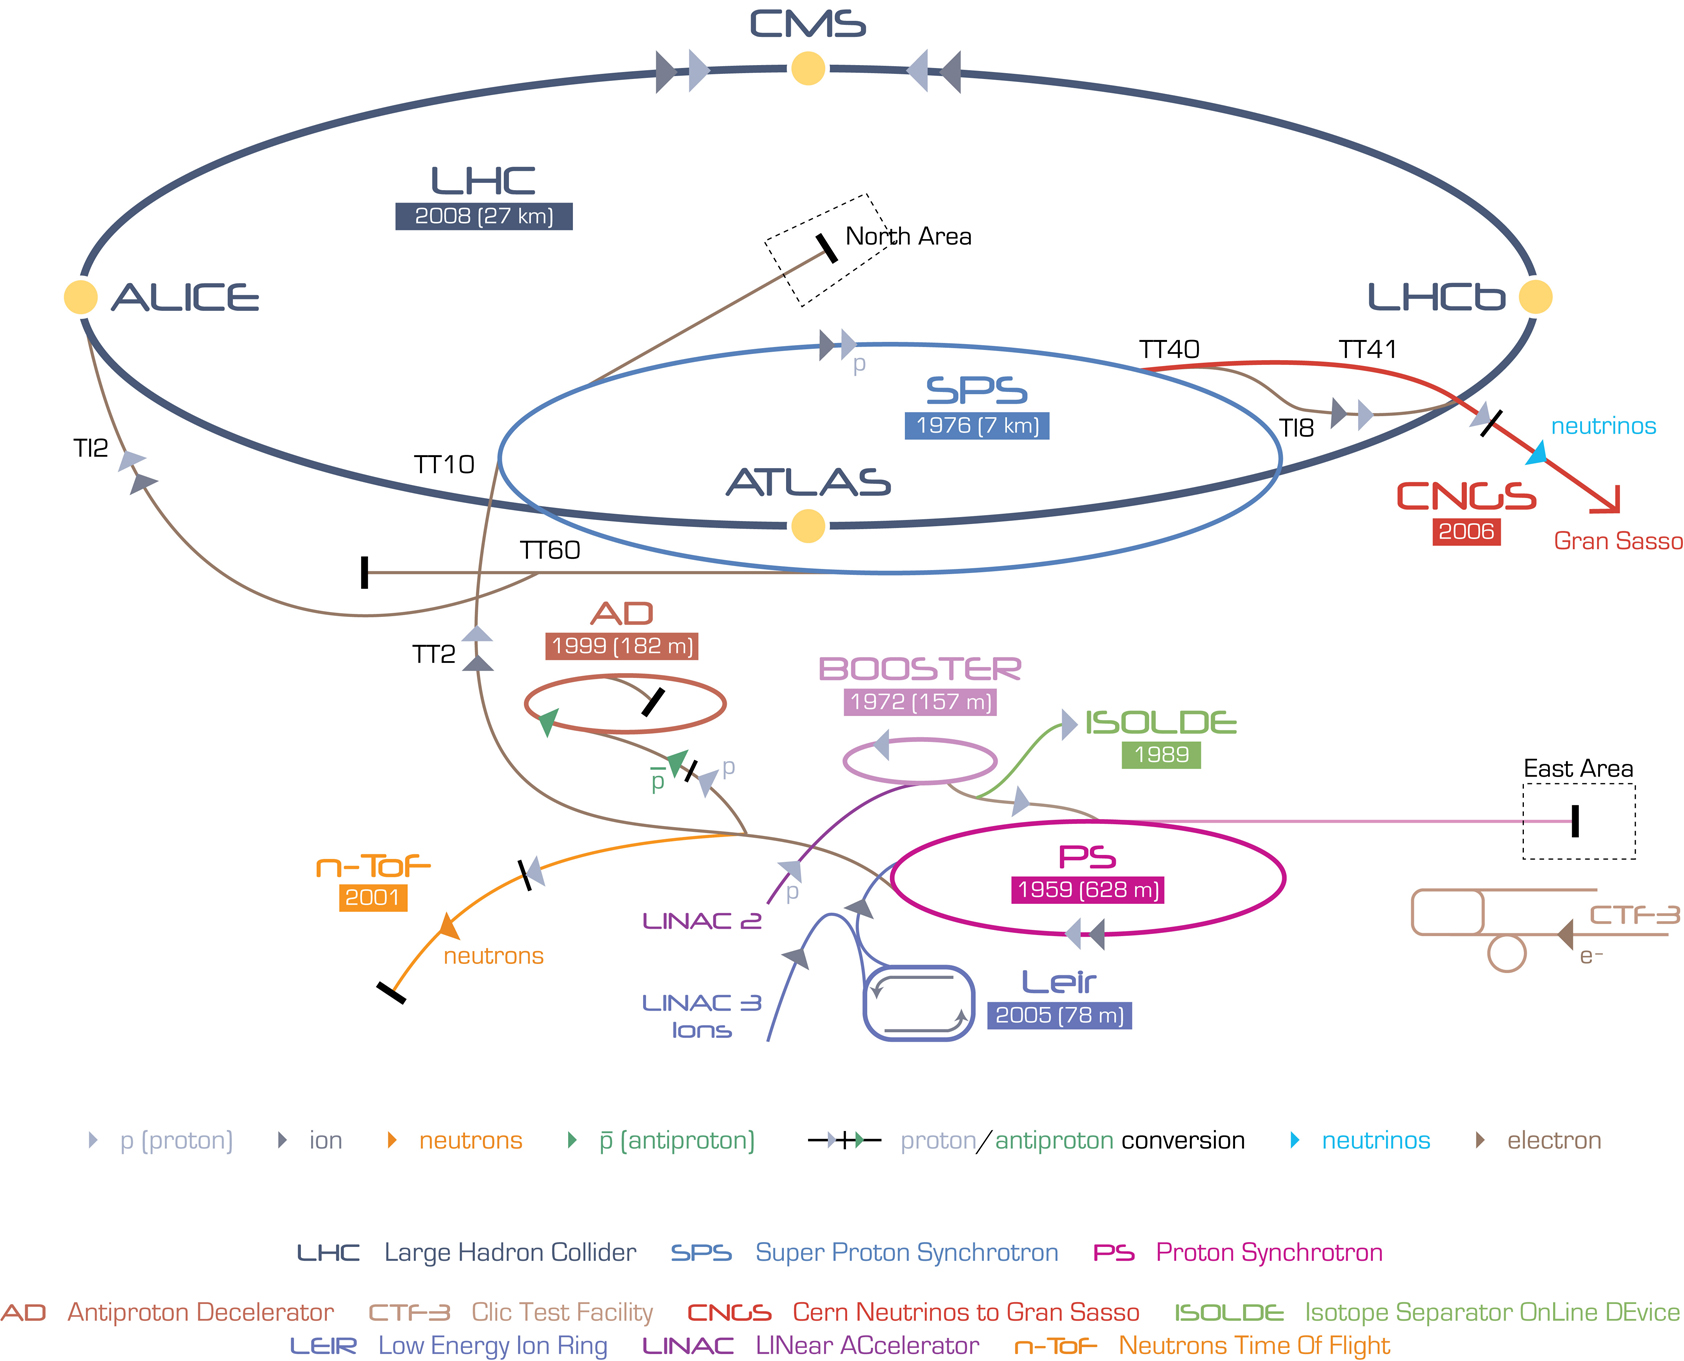
\includegraphics[width=0.9\textwidth]{LHC_fig/Cern-Accelerator-Complex.jpg}
 \caption{The CERN accelerator complex.\label{fig:cernAcc} }
\end{figure}
At this point, the two beams are brought to collide at the four interaction points (IP) in the straight
sections where the LHC's experiments are located. There are two main
purpose experiments located in diametrical opposite locations, the
ATLAS experiment is located at point 1 and the CMS experiment is
located at point 1. There are also two specialized experiments; the
LHCb experiment, which studies B-hadron physics, and the ALICE
experiment, which specializes in studying heavy ion collisions (another type of
collision possible at the LHC). Figure~\ref{fig:LHC} shows an
squematic layout of the LHC.
\begin{figure}
 \centering
 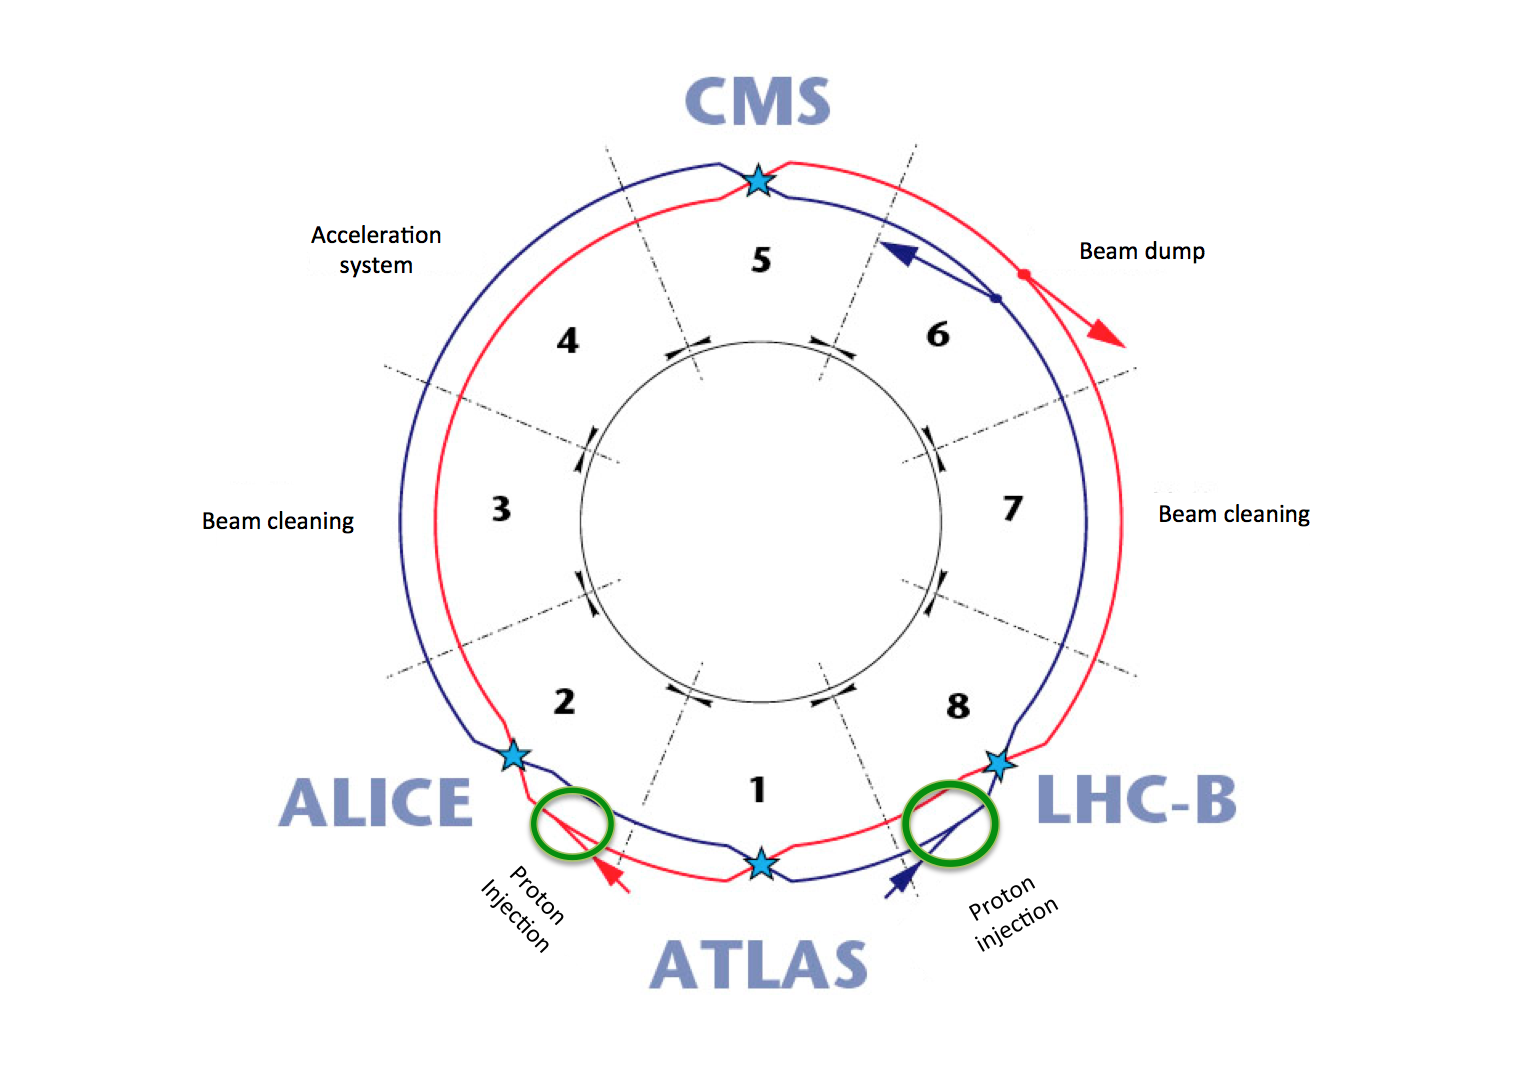
\includegraphics[width=0.9\textwidth]{LHC_fig/LHC_layout.png}
 \caption{The CERN Large Hadron Collider schematic layout.\label{fig:LHC} }
\end{figure}
Due to the small diameter of the tunnel in the arcs
(3.7~m), which complicates the installation of two separate proton
rings, the LHC uses a twin-bore magnet design, proposed in 1971 by
John Blewett at the Brookhaven National Laboratory
(BNL)~\cite{JBlewett} as a cost-saving alternative. 

Since the usage of superconducting magnets a the Intersecting  Storage
Rings at CERN, particle colliders have used them as the default
technology for their operation. However, the main difference is that the LHC's
superconducting magnets operate at a tempareture lower (below 2~K) than the
standard superconducting magnets in other particle colliders
(4-5~K). The LHC ring accomodates 1,232 NbTi main dipole magnets,
cooled down to 1.9 K by using superfluid helium; they operate at fields
above 8~T. The twin-bore desing allow for a common nonmagnetic collar
and iron yoke, as well as common cryogenic system. The core of the
dipole magnet system is enclosed by a cylindrical alloyed low-carbon steel vacuum vessel with an outer diameter of 914\mm and a wall
thickness of 12\mm. Figures~\ref{fig:magnet1} and~\ref{fig:magnet2} show a cross sectional
view and a 3-dimensional visualization of the main dipole magnet
system, respectively.
\begin{figure}
 \centering
 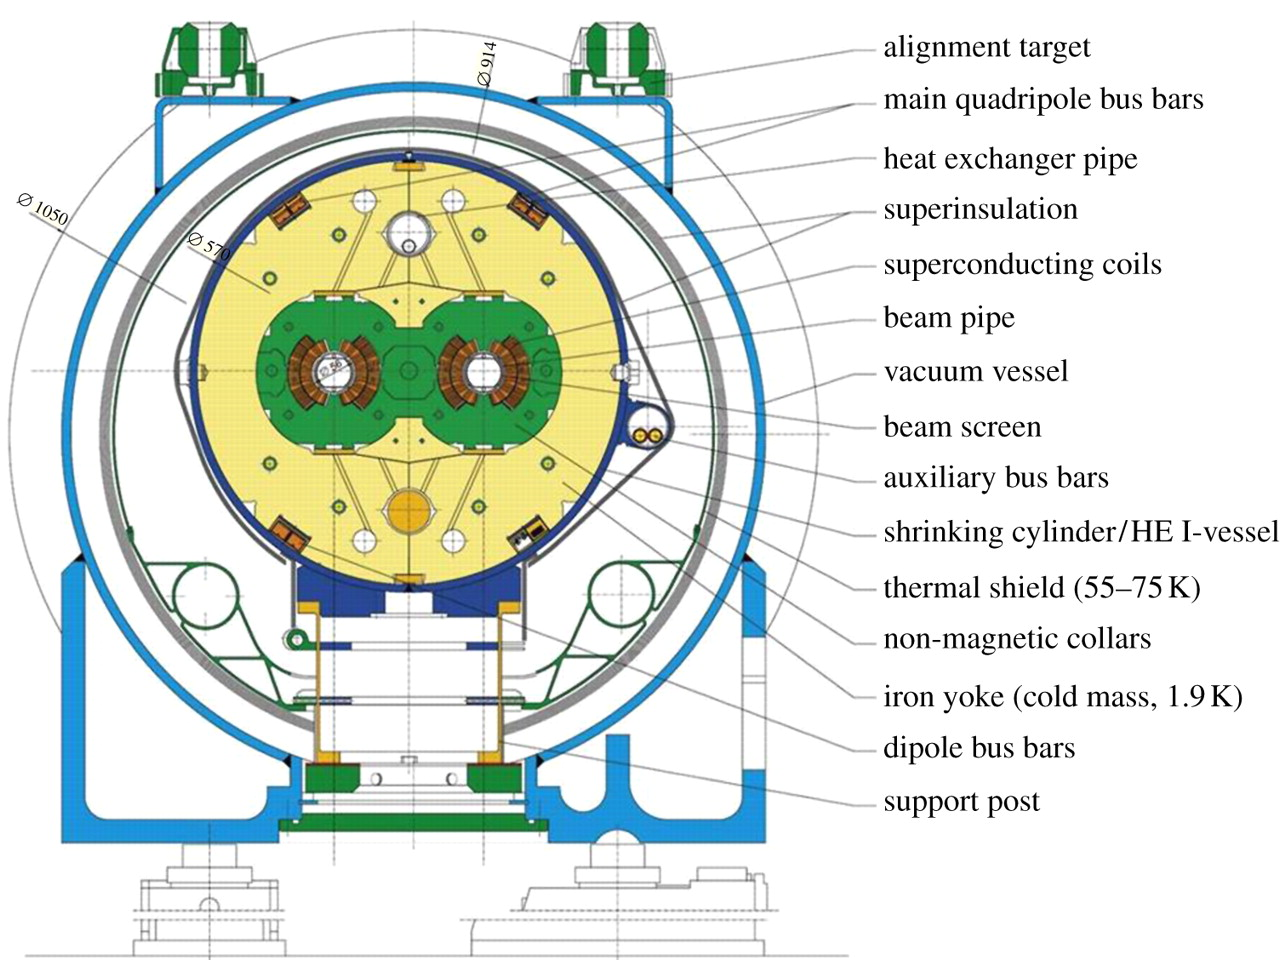
\includegraphics[width=0.9\textwidth]{LHC_fig/ColdMassMagnet.jpg}
 \caption{An schematic cross sectional view of the LHC dipole magnet.\label{fig:magnet1} }
\end{figure}
\begin{figure}
 \centering
 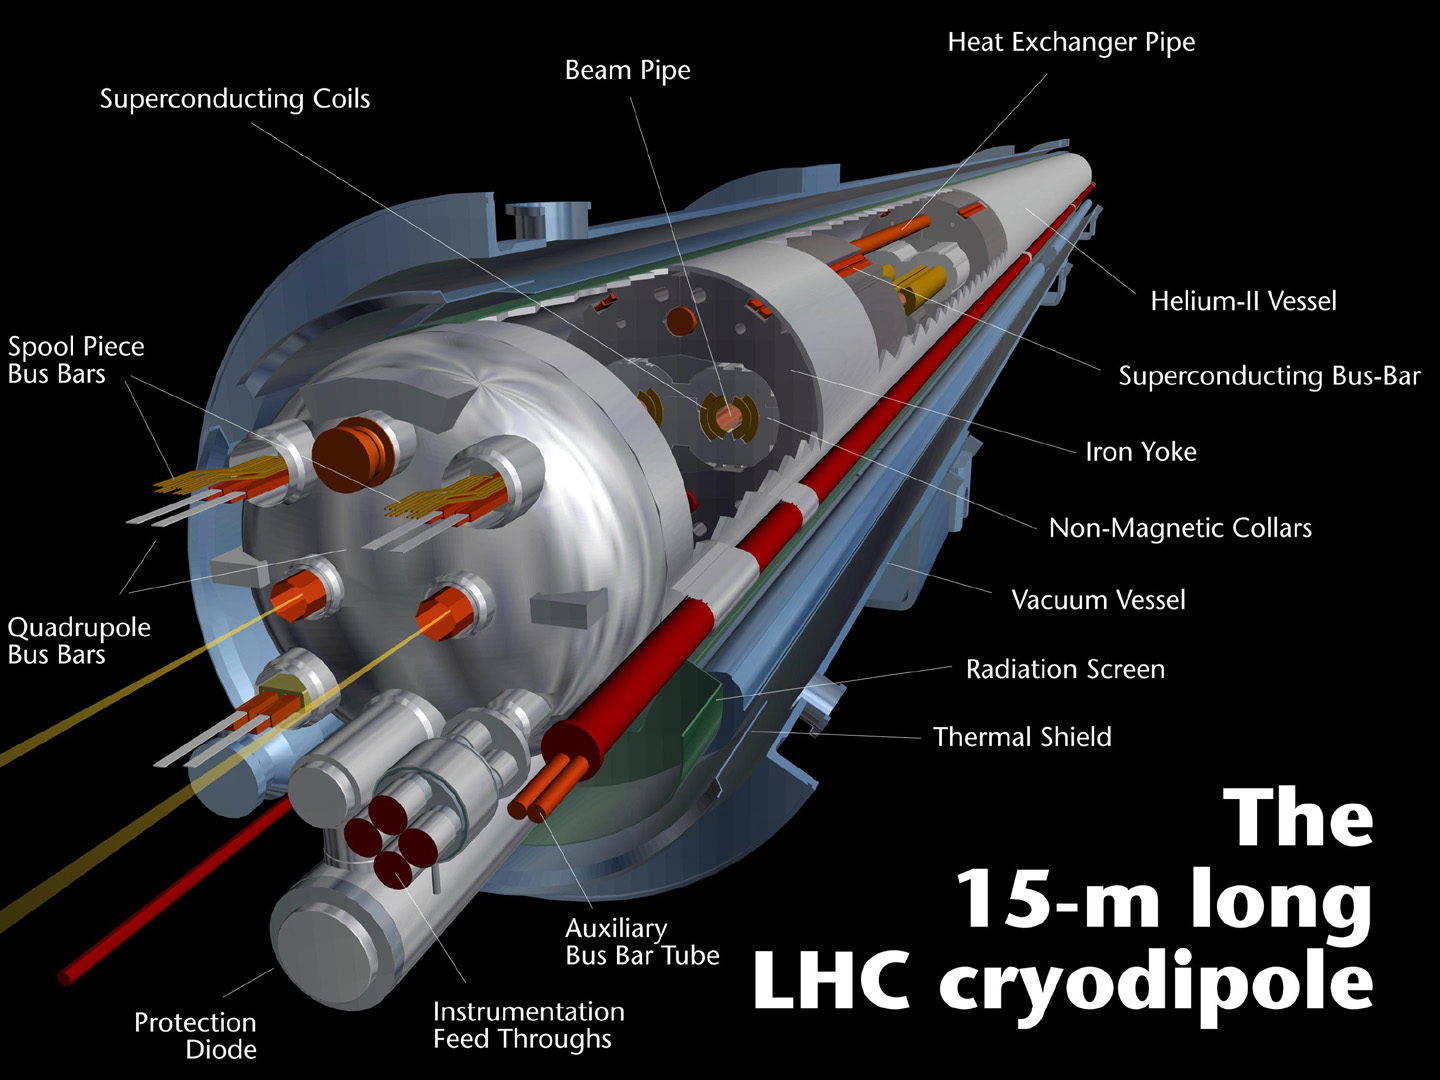
\includegraphics[width=0.9\textwidth]{LHC_fig/cryodipole.jpg}
 \caption{An 3D visualization of a LHC dipole magnet.\label{fig:magnet2} }
\end{figure}

The goal of the LHC program is to reveal the nature of new
physics. The high-energy collision (14\TeV) are a key ingredient to probe new
physics, since new physics could just be present at that energy
scale. However, it is by no means the only ingredient; new physics
will likely have smaller cross sections than that of the known SM
processes and therefore a large number of proton-proton collision is
needed. The number of events for a particular physics process $N_{exp}$
generated in the LHC is the product of the experimental cross section $\sigma_{exp}$
and the integrated luminosity, i.e.
\begin{equation}
N_{exp} = \sigma_{exp}\int\mathcal{L}(t)dt.
\end{equation}
Where $\mathcal{L}(t)$ is the instantaneous luminosity, which depends
on the LHC beam parameters and can be written as~\cite{LHCbeamParam}:
\begin{equation}
\mathcal{L}(t) = \frac{N^{2}_{b}n_{b}f_{rev}\gamma_{r}}{4\pi\epsilon_{n}\beta^{*}},
\end{equation}
where $N_{b}$ is the number of particles per bunch, $n_{b}$ is the
number of bunches per beam, $f_{rev}$ is the revolution frequency,
$\gamma_{r}$ is the relativistic factor, $\epsilon_{n}$ is the
normalized transverse beam emittance, $\beta^{*}$ is the transverse
size of the beam at the IP, and $F$ is the geometric luminosity
reduction factor due to the crossing angle at the IP:
\begin{equation}
F=\left(1+\left(\frac{\theta_{c}\sigma_{z}}{2\sigma^{*}}\right)\right)^{-1/2}
\end{equation}
In the last expression, $\theta_{c}$ is the full crossing angle at the
IP, $\sigma_{z}$ is the rms bunch length, and $\sigma^{*}$ is the
transverse rms beam size at the IP. The designed peak luminosity to be
deliverd the ATLAS and CMS is $\mathcal{L}(t) = 10^{34}$~cm$^-2$~s$^{-1}$.  
Figure~\ref{fig:lumi} shows the integrated luminosity
received by the CMS experiment from 2007 to 2016. 
\begin{figure}
 \centering
 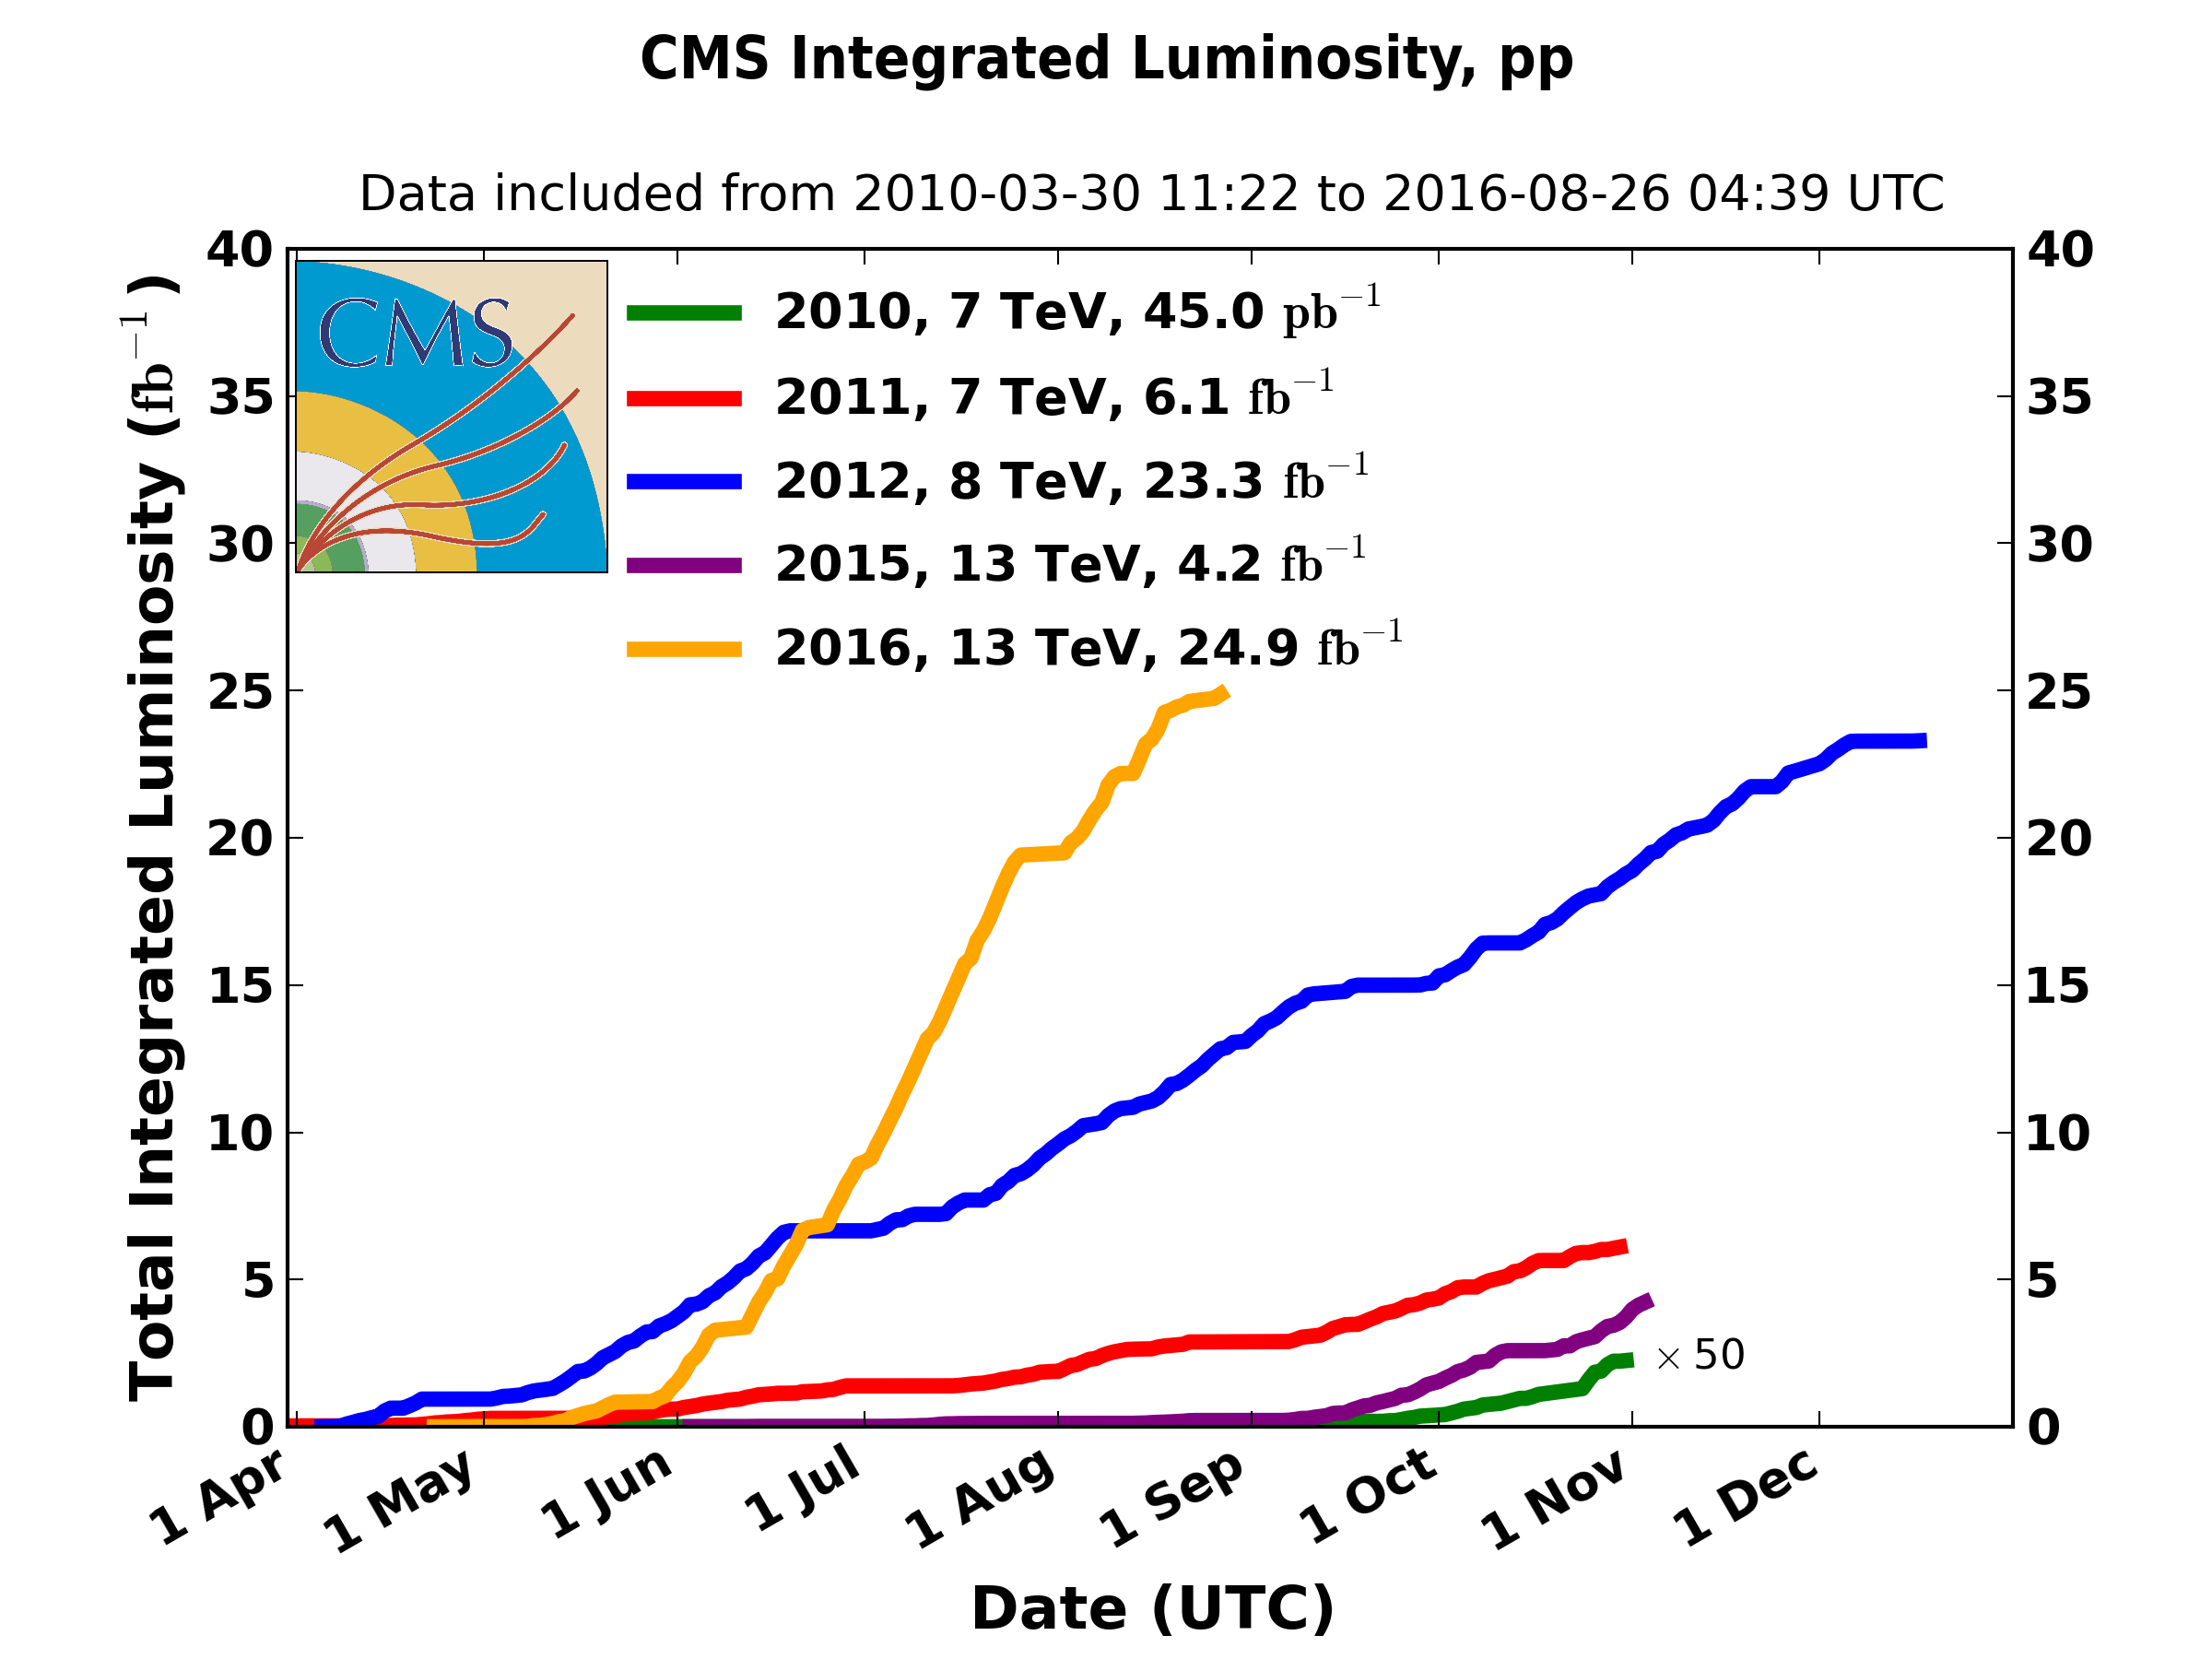
\includegraphics[width=0.9\textwidth]{LHC_fig/int_lumi_cumulative_pp_2.png}
 \caption{Intregated luminosity received by the CMS experiment during the LHC operation.\label{fig:lumi} }
\end{figure}
